\chapter{État final de développement}

L'avancement actuel du projets, permet : 
\begin{itemize}
	\item  d'établir une connexion Ethernet entre le pc hôte et la liseuse
	\item de modifier l'affichage de l'écran e-ink
\end{itemize}

La mis en place de la connexion Ethernet se fait grâce aux modification effectuées sur le système de fichier monté par la liseuse.

% 1 : l'image de la liseuse
%ethernet
	%connection de l'interface reseau eth1 
\section{Fonctionnalités de l'image} %a changer

\subsection{La connexion Ethernet}
La liseuse ne disposant que d'un port USB il faut passer par un module chargeable pour émuler une connexion Ethernet sur ce port.
Ce module est le gadget Ethernet d'android.
Le réseau établi entre la liseuse et le pc est défini statiquement, de plus les adresses MAC des cartes émulées sont fixée par le module.

%capture d'ecran ifconfig
\begin{figure}[]
	\begin{center}
	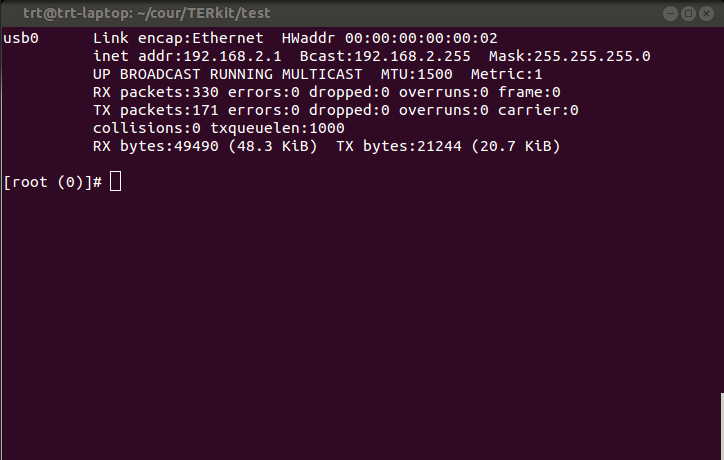
\includegraphics[scale=0.5]{capt_prs_ifconfig.png}	
	\end{center}
	\caption{configuration réseau de la liseuse}
\end{figure}

\begin{figure}[]
	\begin{center}
		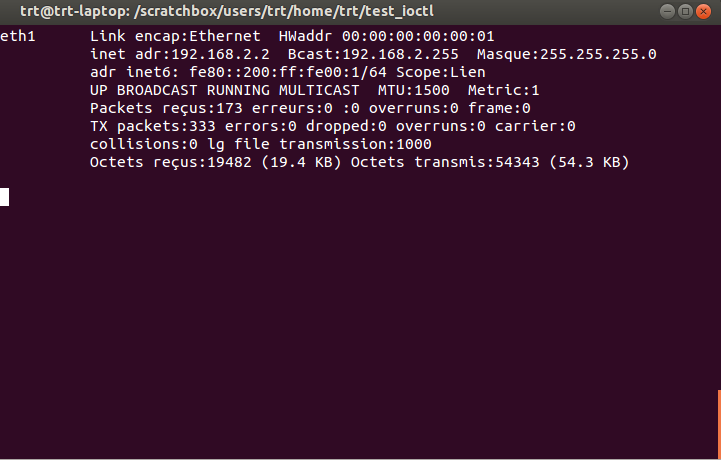
\includegraphics[scale=0.5]{capt_pc_ifconfig.png}
	\end{center}
	\caption{configuration réseau du pc}
\end{figure}
\clearpage
%dropbear
\subsection{L'ajout de ssh}
Pour des raisons pratiques nous avons ajouté à la liseuse la gestion du protocole ssh, afin de pouvoir lancer facilement des commandes sur la liseuse, mais aussi de faciliter la copie de fichiers.
%a voir ci c'est util
Le ssh fonctionne comme une connexion ssh classique.

\section{Programme d'affichage}

La modification de l'écran E-ink peut se faire de deux manières, soit en envoyant les commandes directement au drivers (en utilisant les ioctls), soit en passant par une librairie graphique (ici DirectFB)

\subsection{Affichage via ioctl}

Le programme de test d'affichage via ioctl permet d'envoyer un buffer d'affichage directement dans le framebuffer du driver epdc.
Ici ce buffer est constitué de pixels aléatoire : 
%capture d'écran get_temp

\subsection{Affichage via DirectFB}

Le programme d'affichage via Librairie graphiquegénère le framebuffer en utilisant les primitives de DirectFB.
Le programme de test déssine ici 10 ligne avec points d'arrivée aléatoire.

%capture direct
% 2 : programme d'affichage
%exemple de fonctionnement
